
As mentioned in the previous chapter, the \gls{CBM} will face an unprecedented interaction rate in high-energy physics experiments (up to $10^{7}$~events/s). That number sets also a clear requirement for the detector systems and their corresponding data acquisition. Moreover, due to the huge quantity of incoming data which is closely connected to the storage size, certain design decisions had to be made in order to reduce the raw data coming from the subsystems. To address \gls{CBM} conditions complex triggers would have to be introduced, e.g. signatures of off-target decays of $\Omega$ hyperons. The decay topologies required for the reconstruction of the collisions imply a long trigger latency~\cite{Friese_2017}. In order to realize such a complex trigger logic and reduce the data amount, the raw data needs to be evaluated in software on \glspl{CPU} and/or \glspl{GPU}. The self-triggered readout system implies that the association of data from different detectors to physical collision events must be based solely on their timestamp, which is generated in the frond-end electronic (\gls{FEE}) circuitry. As a result, a central timing system must synchronize the \gls{FEE} elements to sub-nanosecond precision. On the other hand, the typical "event building" action and the high-level trigger are transitioned to the \gls{FLES} ("First-level Event Selector") online compute farm. 


\begin{figure}[!h]
\centering
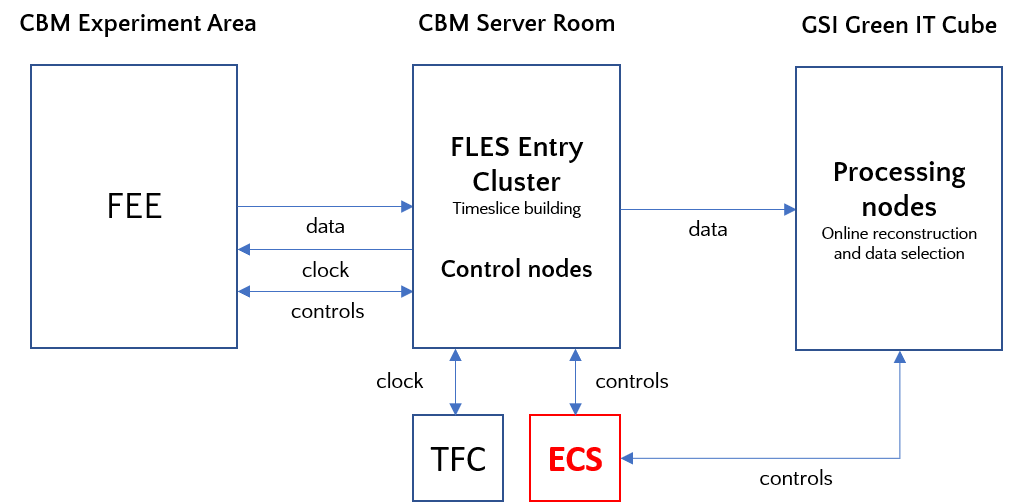
\includegraphics[width=0.8\columnwidth]{Chapter3/Controls/images/online.png}
\caption{Schematics of the CBM readout systems}
\label{fig_controls}
\end{figure}

The readout hardware is connected to the farm via custom-developed optical links that manage clock and time distribution, data transfer, and control communication. The Common Readout Interface (\gls{CRI}) connects the links to the online farm. The CRI forwards the clock and time information obtained from the Timing and Fast Control (\gls{TFC}) system to the detector \gls{FEE}, and also converts the data received from the detector. Figure~\ref{fig_controls} shows the schematic view of the controls and data acquisition chain of the \gls{CBM} experiment. The Experiment Control System (\gls{ECS}) highlighted in red is also the supervisory structure of the Detector Control System (\gls{DCS}) which controls and monitors the subsystems. The next sections focus on the software components related to the \gls{ECS}, and a detailed explanation of the experiment control with its design. Nevertheless, the main focus is put on the \gls{DCS}. An introduction to the modern control system frameworks is given, together with a detailed explanation of the functionalities of the specific software components. 
%\newpage
\section{Controlling a HEP experiment}

Modern \gls{HEP} experiments require complex control systems which are crucial to the successful operation of the installment. Proper implementation of such systems ensures higher safety margins and enhanced data production quality. 
Figure \ref{fig_sim} depicts the targeted controls architecture of the future \gls{CBM} experiment. It consists of different \footnote{A software agent is a persistent, goal-oriented computer program}{software agents} with clearly defined tasks. During the Phase - 0 experiment of the \gls{CBM} (\gls{mCBM}) some parts of the future \gls{ECS} were tested. The respective parts of the controls have been tested in a standalone mode, which means that there hasn't been any structured communication between \gls{DCS}, Device Control Agent (\gls{DCA}), and Experiment Control System (\gls{ECS}). Nevertheless, for the final experiment the detector control system should provide the information on the detector state to the agent(s) residing at a higher position in the control hierarchy, and also request the state of the~\gls{DAQ}.
\begin{figure}[!h]
\centering
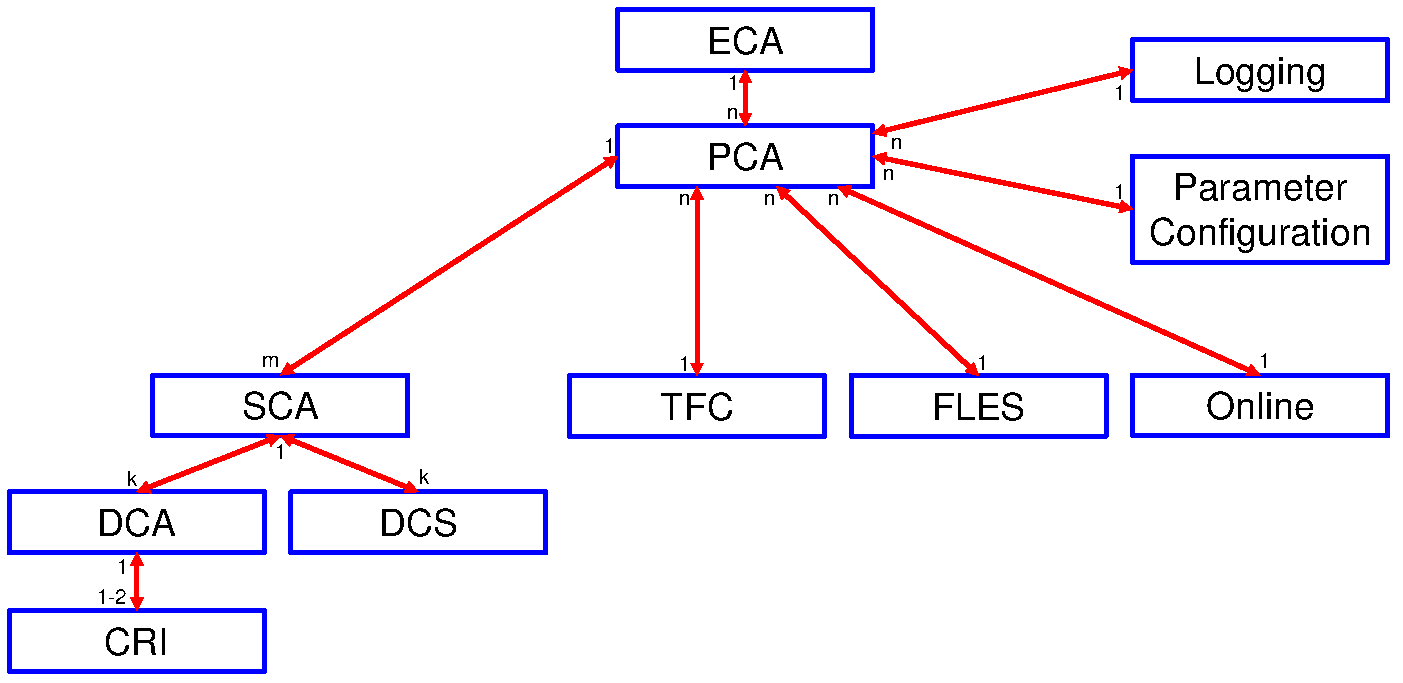
\includegraphics[width=0.8\columnwidth]{Chapter3/Controls/images/AgentsRelations_V2.pdf}
\caption{\gls{ECS} core agent relations}
\label{fig_sim}
\end{figure}

 In the next sections, the main features of the control agents are discussed, in particular those that can influence \gls{DCS} (Partition Control Agent (\gls{PCA}), System Control Agent (\gls{SCA}), and \gls{DCA}). Apart from the mentioned agents, the following components are expected to run: 
 \begin{itemize}
     \item Logging and monitoring system - state or configuration changes should be documented for possible revision,
     \item First Event Selector network - \gls{DAQ} software controlling the data readout and timeslice building,
     \item Online processing - software receiving the data from the FLESnet and processing it,
     \item Time and Fast Control (\gls{TFC}) - hardware source of timing information.
 \end{itemize}
\section{Experiment Control System}\label{sssAgents}

The highest supervisory element of the control strategy is the Experiment Control Agent 
(\gls{ECA}). It is the top layer of the \gls{ECS} core, which should be constantly running and keeping track of the  partitions, of the systems in partitions, and of the systems out of partitions. Partition is a component of the \gls{ECS} describing the combined state of a set of detector systems participating in a common readout. It is used to segment the readout and data flow. It also manages the states of "Central systems," which do not have partition-level states (e.g. \gls{TFC}, \gls{FLES} in case it does not use internal partitions).  It provides the address and port required by agents to establish the \footnote{asynchronous messaging library \cite{zeromq}}{0MQ} sockets and build the \gls{ECS} structure upon request. The \gls{PCA}, is the bottom layer of the \gls{ECS}, which tracks the state and controls a set of detector systems plus all needed central systems. Multiple partitions can run concurrently, potentially allowing for parallel runs with independent detector system sets. 

The \glspl{PCA} also hold internal instances of the necessary System Control Agent \gls{SCA} interfaces, which are responsible for:
\begin{itemize}
 \item holding a copy of the current state of the \gls{SCA},
 \item periodic ping of the \gls{SCA} to ensure early disconnection detection,
 \item sending requests to the \gls{SCA} and receiving the replies,
 \item Monitoring the \gls{SCA} broadcast channel for unexpected/unrequested state changes.
\end{itemize}
These should not be confused with the \gls{SCA}, which are in separate processes (the list will be dynamic and generic at \gls{PCA} level, and can depend on the systems participating in the readout activities):

\begin{itemize}
 \item Time zero (T0), also known as Start Detector or Beam Monitor \gls{BMON})
 \item Micro-Vertex Detector (\gls{MVD})
 \item Silicon Tracking System (\gls{STS})
 \item Ring Imaging CHerenkov (\gls{RICH})
 \item MUon CHambers (\gls{MUCH})
 \item Transition Radiation Detector (\gls{TRD})
 \item Time Of Flight (\gls{TOF})
 \item Beam Fragment Timing Counter (\gls{BFTC})
 \item Projectile Spectators Detector (\gls{PSD})
\end{itemize}

\subsection{System Control Agent and its role}
The subsystem-specific \gls{SCA} should manage communication both with the detector-specific agents and with the higher supervisory entities of the \gls{ECS}. Moreover, the \gls{SCA} should provide higher control levels with the global state whenever it's requested, handle any changes reported by a detector (tracking the state), and provide an interface for the shift crew to monitor the state of the system. 

Two main links of the \gls{SCA} include:
\begin{itemize}
    \item Detector control system - Experimental Physics and Industrial Control System \gls{EPICS}~\cite{EPICS} based distributed control system which controls and monitors all the hardware connected to the specific detector,
    \item Device Control Agent (\gls{DCA}) - this agent controls almost all logic on the \gls{CRI} board (excluding the \gls{FLIM} section and direct memory access data path). \gls{DCA} provides a high-level interface for the higher layers of the control architecture, collectively referred as \gls{EDC}. 
\end{itemize}










